\section{Deep Neural Networks}
The \textbf{philosophy} on which \textbf{Deep Learning} relies is to provide a new method for selecting and extracting the features that are provided as input to a classifier, by exploiting the data of the training set. 

More specifically, instead of selecting manually good features and then using them to feed a classifier, Deep Neural Networks learn from the data a \textbf{feature hierarchy} from the initial pixel image in order to obtain a \textbf{classifier}: each layer extracts features from the output of the previous layer, and finally the training phase involves all the layers, jointly.
\image{img/deep_learning}{Example of deep learning process.}{0.75}

As we can see, each layer of the pipeline learns to extract features from the image/video/pixels (in general, from the data we have), and the \textbf{deeper} the layer is, the \textbf{more abstract} the extracted features are.

\subsection{Shallow vs Deep Networks} \textbf{Shallow architectures} are \textbf{inefficient} at \textbf{representing deep functions}, since they are characterized by a limited number of hidden layers. A shallow network with a large single hidden layer can fit any function (i.e. it is a universal approximator), but on the other hand this increases significantly the number of parameters. 

A \textbf{deep network} can \textbf{fit} functions \textbf{better} with less parameters than a shallow network, increasing the number of hidden layers but decreasing the number of required parameters. Deep networks try to simulate the brain's behavior, in which the electric signals propagate across different layers.
\image{img/shallow_vs_deep}{Shallow vs Deep Networks.}{0.78}

Another important aspect to notice is the \textbf{improvement} in \textbf{performance} with the presence of more data.
\image{img/performances}{Performances improves with more data.}{0.6}
As we can see, in the case of basic ML algorithm after a certain amount of data the performance does not increase anymore: in SVM's, for example, this phenomenon happens since the decision boundary obtained by the model only depends on the support vectors, so increasing the size of the training set does not change the accuracy.

The \textbf{usage} of deep networks is not a \textbf{recent} idea (indeed, these networks are fairly old), but it has been made possible only nowadays thanks to the fact that we have \textbf{more data} and \textbf{more computing power}. In particular, the advances in the field of \textbf{GPUs} have made using deep networks way more feasible than before.

\paragraph{Image classification.} The \textbf{image classification} problem consists in predicting a single label (or a probability distribution over all the possible labels to indicate our confidence, as per the following example) for a given image. Images are 3-dimensional arrays of integers from 0 to 255 of size Width x Height x 3. The 3 represents the three color channels Red, Green and Blue.
\image{img/image_classification}{Image classification example.}{0.5}
In image classification, the most important \textbf{challenges} are the following ones:

\image{img/challenges}{Challenges in image classification.}{0.95}
In order to face these challenges, what we need is a data-driven approach in which we have thousands of categories and hundreds of thousand of images for each category.\\
As it is possible to understand, there's a difference between \textbf{traditional approaches} and \textbf{deep learning}. Indeed, in the first one we extract \textbf{meaningful features} from images through a \textbf{manual} process, while in the second case everything happens \textbf{automatically} thanks to a sequence of \textbf{layers} in which the final ones are useful for classification.

\paragraph{Inspiration from biology.} As we introduced before, functioning of Deep Neural Networks is highly inspired from biology, and in particular the architecture resembles the one in the visual cortex of the brain. Indeed, biological vision is hierarchically organized, and the basic component of this hierarchy is the \textbf{retina}. The cells of the retina are arrayed in discrete layers, with the \textbf{photoreceptors} at the top of them that are divided into:

\begin{itemize}
    \item \textbf{Rods}, which are sensitive to the intensity of the light and to movements;
    \item \textbf{Cones}, which are sensitive to colors.
\end{itemize}

We define \textbf{receptive field} the region of the visual field in which light stimuli evoke responses of a given neuron. In terms of Deep Networks, this makes a distinction between \textbf{fully connected Neural Networks}, in which each neuron is connected to all the neurons of the previous layer, and \textbf{sparsely connected Neural Networks}, in which each neuron is characterized by a corresponding \textbf{receptive field}, i.e. it is connected only to a subset of neurons of the previous layer.

The \textbf{take-home} message of this digression is that the \textbf{visual system} is a \textbf{hierarchy} of \textbf{features detectors}.

\paragraph{The Neocognitron (1980).} The first example example of self-trained network for feature learning was the \textbf{Neocognitron}, introduced in 1980.

\subsection{Convolution}
The \textbf{convolution} is a mathematical operation that takes as input an \textbf{image}, i.e. an array of pixels, and a 3x3 array of numbers (called \textbf{convolution filter}), and applies the 3x3 array in a certain portion of the image, and computes the summation of the products between the pixels of the image and the one in the filter. 

\begin{figure}[h!]
		\centering
        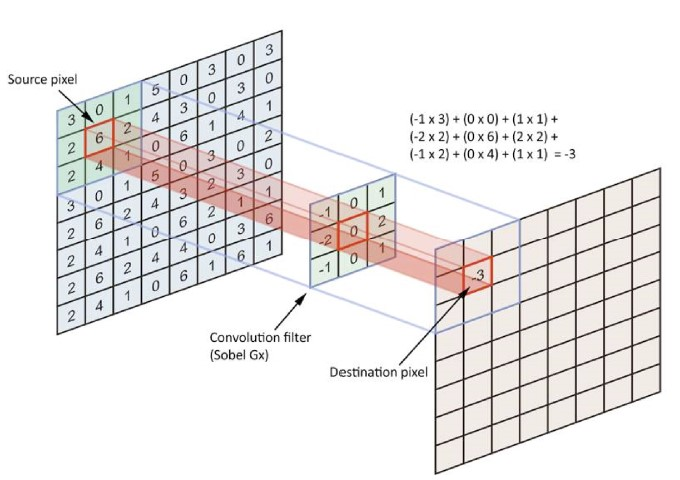
\includegraphics[scale = 1.5]{img/convolution.jpg}
		\label{mi}
        \caption{Example of convolution}
\end{figure}

Notice that there exist many type of filters, which differ for their values.

\begin{figure}[h!]
		\centering
        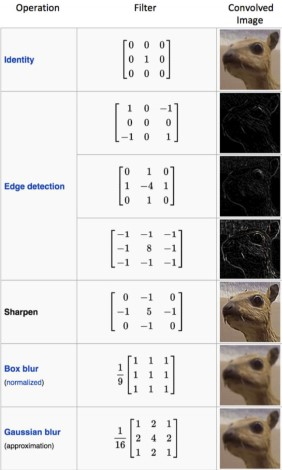
\includegraphics[scale = 1.5]{img/filters.jpg}
		\label{mi}
        \caption{Types of filters}
\end{figure}

\subsubsection{Stride and Padding}

The \textbf{stride} quantity denotes how many steps we're moving in each step of convolution, and the default value is 1. In order to maintain the dimension of the output the same as the one of the input, we use \textbf{padding}, which is the process of adding 0s to the input matrix symmetrically.

\begin{figure}[h!]
		\centering
        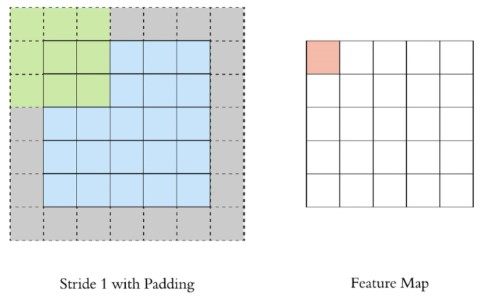
\includegraphics[scale = 1.5]{img/stride and padding.jpg}
		\label{mi}
        \caption{Stride $= 1$ with padding $ = 1$}
\end{figure}

In this sense, \textbf{stride} and \textbf{padding} can be used to \textbf{adjust} the \textbf{dimensionality} of the \textbf{data} effectively.

\subsubsection{Multiple channels}

In the case in which the convolution is applied to an image with multiple channels, we can use a different filter for each channel, and then combine the results into a single output matrix.

\begin{figure}[h!]
		\centering
        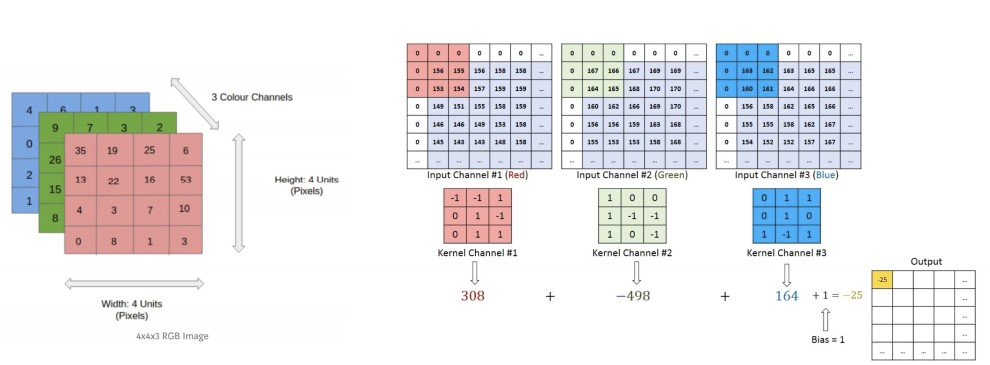
\includegraphics[scale = 1.5]{img/convolution with multiple channes.jpg}
		\label{mi}
        \caption{Example of convolution of an image with multiple channels}
\end{figure}

\subsubsection{Gaussian filter}

A very famous filter used in convolution is the Gaussian filter, which basically computes a weighted average of the pixels of the image, where the weights are proportional to the distance with the central pixel.

\begin{figure}[h!]
		\centering
        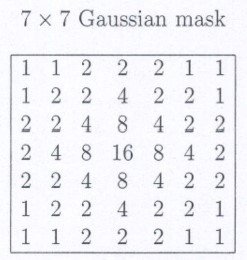
\includegraphics[scale = 1.5]{img/gaussian filter.jpg}
		\label{mi}
        \caption{Example of 7x7 Gaussian filter}
\end{figure}

The result of applying a Gaussian filter to an image is to obtain a \textbf{blurred version} of the image: the larger the filter, the more blurred the output image is.

\subsubsection{Convolution for edge detection and other problems}
An important application of the convolution operation is \textbf{edge detection}, i.e. the problem of determining the contour of an object.

\begin{figure}[h!]
		\centering
        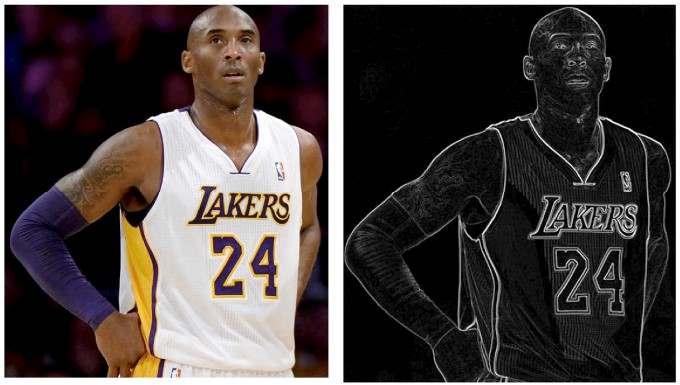
\includegraphics[scale = 1.5]{img/edge detection.jpg}
		\label{mi}
        \caption{Edge detection problem}
\end{figure}

Some of the most famous filters that are used in edge detection are \textit{Roberts operator}, \textit{Sobel operator} and \textit{Prewitt operator}. Other filters are used for different tasks, e.g. \textit{HoG} is used for the problem of \textit{pedestrian recognition} etc..

\subsection{Convolutional Neural Networks (CNNs)} 
\subsubsection{Fully-connected and sparsely-connected networks}
A neural network can be defined as a \textbf{fully-connected network} or a \textbf{locally-connected network}. In a fully-connected network, each neuron of each layer is connected to every neuron in the previous one, and each connection has its own weight. In this sense, the number of parameters is huge.

Conversely, in a locally-connected layer, each neuron is only connected to a \textbf{few nearby neurons} in the previous layer, and the same set of weights (and local connection layout) is used for each neuron. The typical use case for locally-connected layers is for image data where, as required, the \textbf{features} are \textbf{local} (e.g. a "nose" consists of a set of nearby pixels, which are not spread across the whole image), or in general in applications where the local connections capture local dependencies. The smaller number of connections and weights makes local-connected layers \textbf{relatively cheap} in terms of memory and computing power needed.
\image{img/fully_local}{Fully vs local-connected networks.}{0.75}

\subsubsection{Weight sharing}

Before providing the definition of \textbf{CNN}, we now define the concept of \textbf{weight sharing}. This concept is based on the following reasonable assumption: if one feature is useful to compute at some spatial position $(x_1, y_1)$, then it should be useful to compute at a different position $(x_2, y_2)$. In this way we can dramatically reduce the number of parameters.

\begin{figure}[h!]
		\centering
        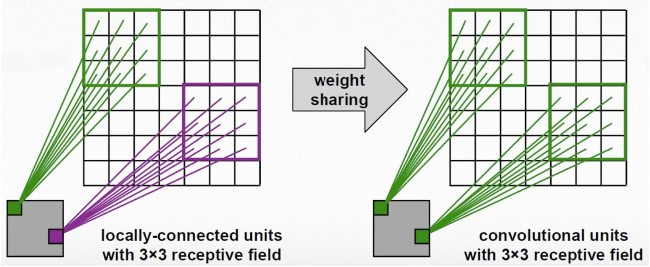
\includegraphics[scale = 1.5]{img/weight sharing.jpg}
		\label{mi}
        \caption{Weight sharing operation}
\end{figure}

As we can see, in the first case we have neurons detecting different features (i.e. different weights in the receptive fields), while in the second case the two neurons have the same weights in the corresponding receptive fields, so they're detecting the presence of the same feature in different portions of the image. Note that while in the traditional convolution operation the weights are applied directly to the pixels of the image, in this case they become the weights of the connections of the receptive fields. 

\subsubsection{Definition of CNN}
A \textbf{Convolutional Neural Network (CNN)} is a \textbf{multi-layer feed-forward neural network} characterized by \textbf{local connectivity} (i.e. neurons with the correspondent receptive field) and \textbf{weights} that are \textbf{shared} across spatial positions. Normally, \textbf{several filters} are \textbf{packed} together and \textbf{learned automatically} during training.
\image{img/trainableFilters}{Using Several Trainable Filters.}{0.75}

\paragraph{Pooling.}\textbf{Pooling} is a way to \textbf{simplify} the network architecture, by downsampling the \textbf{number of neurons} resulting from the filtering operations. An example of pooling technique is the \textbf{max pooling}, in which the \textbf{image} is \textbf{partitioned} in small squares and for each square the pixel with \textbf{maximum value} is taken.
\image{img/max_pooling}{Max Pooling.}{0.6}
As we can see in the next image, a \textbf{Deep Convolutional Neural Network} is a \textbf{combination} of \textbf{feature extraction} and \textbf{classification processes}:

\begin{itemize}
    \item The \textbf{input} of the network is represented by an \textbf{image};
    \item The \textbf{input layer} is followed by some \textbf{locally-connected layers} that \textbf{extract features} from the image. As we can see, this feature extraction phase is mainly composed of \textit{convolution} and \textit{subsampling} operations;
    \item Finally, a \textbf{fully-connected layer} provides the \textbf{classification} of the input image.
\end{itemize}

\image{img/extraction_and_classification}{Combining Feature Extraction and Classification.}{0.7}

\subsection{AlexNet (2012)} 
The first example of Deep Convolutional Neural Network we examine is the \textbf{AlexNet}. This architecture was developed in 2012 for solving the problem of \textbf{image classification}, and it was trained using the \textit{ImageNet} dataset, comprising 1,000 categories, 1.2M training images and 150k test images. The results were astonishing, since the error was reduced by 22\% in only 3 years.

More specifically, this architecture is not so different from the one of the \textit{Neocognitron}, or from the one proposed by LeCun in 1998, but this was much larger. AlexNet is composed of \textbf{8 layers} as per the following schema:
\imageb{img/alexNetLayers}{0.18}
The first thing we can notice are that:

\begin{itemize}
    \item The \textbf{input} is given by an \textbf{image};
    \item The \textbf{first 5 layers} are used for \textbf{extracting features} for the classification phase: as we can see, we have a combinations of \textit{convolution} and \textit{pooling} operations;
    \item \textbf{Layer 6 and 7} provide the \textbf{classification} of the input: as we can see, in this case we exploit fully connected layers;
    \item The \textbf{output layer} is represented by a \textbf{Softmax} function, which provides a probability distribution of the classes of the input image.
\end{itemize}

\image{img/alexNet}{AlexNet architecture.}{0.8}

Diving deeper into these layers' characteristics, we can notice that:
\begin{itemize}
	\item \textbf{1st layer:} we have 96 kernels of size $(11 \times 11 \times 3)$, which are applied to the input image: the results is then convolved (stride = 4) and pooled. Notice that the output of the first layer has not a width of 96, and this is because it was splitted into two different outputs, each with width equal to 48. By looking at the top-9 patches for one filter we can observe that the neurons are very sensitive for colors and geometric forms, so they're very simple;
	\item \textbf{2nd layer:} we have 256 kernels of size $(5 \times 5 \times 48)$, which are then normalized and pooled. Notice the 256 kernels are given by two blocks of 128 kernels. Here the neurons distinguish more abstract features, and this process continues as we go deeper in the Deep Network;
	\item \textbf{3rd layer:} we have 384 kernels of size $(3 \times 3 \times 256)$;
	\item \textbf{4th layer:} we have 384 kernels of size $(3 \times 3 \times 192)$;
	\item \textbf{5th layer:} we have 256 kernels of size $(3 \times 3 \times 192)$;
	\item \textbf{6th layer:} we have a fully connected layer with 4096 neurons;
	\item \textbf{7th layer:} we have a fully connected layer with 4096 neurons;
	\item \textbf{8th layer:} we have a 1000-way \textbf{SoftMax} output layer, i.e. 1 output for each of the possible classes, since it provides a probability distribution.
\end{itemize}
While training the network, two independent GPUs run in parallel, in order to speedup the training process. This is the reason why the output of the first layer was splitted. 

The last \textit{SoftMax} layer gives as output:
$$y_i = \frac{e^{z_i}}{\sum_j e^{z_j}}$$
, where $z_i$ represents the output of the network and it is defined as:

$$
z_i = w_i^T \cdot x
$$

\begin{figure}[h!]
		\centering
        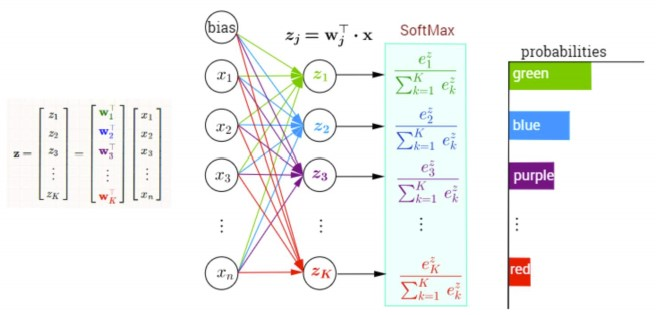
\includegraphics[scale = 1.5]{img/softmax.jpg}
		\label{mi}
        \caption{Output of the SoftMax function}
\end{figure}

Since the output of the SoftMax is a probability distribution over all the possible classes of the training set, we can compute the \textbf{Cross-entropy loss} between the actual output and the desired one, in order to measure the quality of the model.

\subsection{ReLU} \textbf{ReLU} is an acronym that stands for \textit{Rectified Linear Unit}. ReLUs are used to solve the \textbf{problem} that \textbf{sigmoid activation} takes only values in $(0,1)$. While propagating the gradient back to the initial layers, it tends to get closer and closer to $0$ (this phenomenon is called \textit{vanishing gradient}, and it intensifies when the number of layers is high). From a practical perspective, this slows down the training procedure of the initial layers of the network. Indeed, with sigmoid the gradient will be close to 0 and the algorithm won't learn. In order to speed up the learning phase, ReLU is used.
\image{img/relu}{Comparison between sigmoid and ReLU functions.}{0.8}
It is also possible to notice that ReLU reaches the \textbf{same results as sigmoid}, but \textbf{much faster}. In the following image, the solid line represents the convergence of a 4 layer CNN with ReLUs, while the dashed line represents an equivalent network with $tanh$ neurons. It can be noticed that the CNN with \textbf{ReLUs converges six times faster}.
\image{img/relu2}{Convergence of ReLU neurons.}{0.4}

\subsection{Mini-batch Stochastic Gradient Descent} 
We recall that in the back-propagation algorithm we can have either the \textbf{on-line} implementation or the \textbf{off-line} one: in the first one, the weights are updated at any presentation of an example of the training set, while in the second one the gradient is computed exactly. We indicated the \textbf{stochastic gradient descent} as a possible compromise between the two approaches, now we introduce the \textbf{mini-batch stochastic gradient descent}, which is defined as follows:

\begin{enumerate}
	\item Sample a batch of data (the dimension is an hyperparameter to choose), i.e. a subset of the training set;
	\item Perform the forward pass and compute the loss;
	\item Perform the backward pass to compute the gradients;
	\item Update the weights using the gradient (by minimizing the loss).
\end{enumerate} 

Notice that, like in stochastic gradient descent, the use of random samples helps in finding global minima.

\subsection{Data augmentation}
The easiest and most common method to \textbf{reduce overfitting} on image data is to \textbf{artificially enlarge} the \textbf{dataset} using \textbf{label-preserving transformations}. This technique is used to make the dataset more robust. \textbf{AlexNet} uses two forms of \textbf{data augmentation}:
\begin{itemize}
	\item The first form consists in \textbf{generating image translations} and \textbf{horizontal reflections} (translations, scaling or rotations of the images);
	\item The second form consists in \textbf{altering the intensities} of the \textbf{RGB channels} of the \textbf{training images} (introduce random noise inside the images). 
\end{itemize}

\image{img/dataAugmentationBoys}{Data augmentation: translation, reflection, scaling, rotation, RGB noise.}{0.35}

\subsection{Dropout} This technique is exploited in order to have a network with \textbf{more generalization power}, and it consists on \textbf{randomly dropping out some neurons} during the back-propagation algorithm, by setting to 0 the output of that neuron with probability $0.5$. The neurons which are \textit{"dropped out"} in this way do not contribute to the forward pass and do not participate in back-propagation. Every time an input is presented, the neural network samples a different architecture, but all these architectures share weights.\\
Dropout reduces complex co-adaptations of neurons, and it forces the network to find different "roads" in order to produce the outputs, resulting in a more robust network.
\image{img/dropout}{Dropout results}{0.55}

\subsection{Feature analysis}
A well trained Deep Convolutional Neural Network is an excellent \textbf{feature extractor}: in particular, the idea is to chop the network at a desired layer and use the output as a feature representation to train a SVM on some other dataset. Here we show some results.

\begin{figure}[h!]
		\centering
        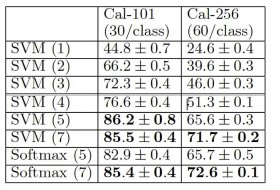
\includegraphics[scale = 2.0]{img/feature extraction.jpg}
		\label{mi}
        \caption{Results using CNN's as feature extractors}
\end{figure}

The parenthesis indicates the layer at which the output is taken: as we can see, the accuracy of the classifier increases as we choose features from more layers, underlying the property of CNN's of learning more and more accurate features as the number of layers grow.

\subsection{CNN's in computer vision tasks}
After 2012, many CV tasks were addressed using CNN's, for example:

\begin{itemize}
    \item \textbf{Semantic segmentation}: in this case the input is an image, and each pixel is classified with a label;
    \item \textbf{Classification and localization}: in this case we assume that the input image contains a single prominent object, and the output consists of single label of the object (standard classification) together with the position of the object;
    \item \textbf{Object detection}: in this case we detect all the objects in an image, where the number is not known in advance;
    \item \textbf{Instance segmentation}: this problem represents a variation of the image segmentation problem, and it consists of labeling each pixel differentiating between objects having the same label.
\end{itemize}

\begin{figure}[h!]
		\centering
        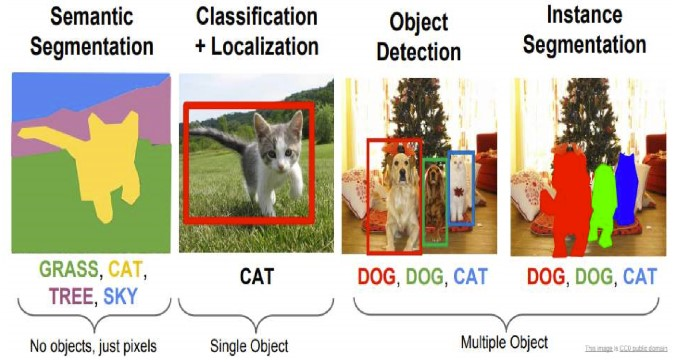
\includegraphics[scale = 1.5]{img/cv tasks.jpg}
		\label{mi}
        \caption{Computer vision problems}
\end{figure}

In general, the adoption of CNN's for solving such problems is having a huge impact in the results.

\subsection{Recurrent Neural Networks}
If we consider the problem of \textbf{image captioning}, i.e. of providing a textual description of the content of an image, it is clear that the usage of a \textbf{feed-forward neural network} does not help in this case, since the output depends on the input. For this reason, we have to exploit \textbf{recurrent neural networks}.

\begin{figure}[h!]
		\centering
        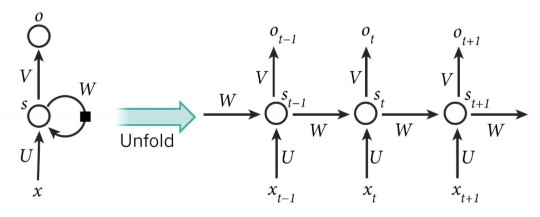
\includegraphics[scale = 1.5]{img/rnn.jpg}
		\label{mi}
        \caption{Recurrent neural network}
\end{figure}

The image shows the unfolding of the simplest recurrent NN, i.e. the one composed of a single hidden layer. Notice that this architecture is different from a feed-forward NN for two main reasons:

\begin{itemize}
    \item We do not know in advance the number of layers;
    \item In a feed-forward NN we have different weights between the layers, while in this case we only have 1 batch of weights for each connection.
\end{itemize}

If we denote with $W_{xh}$ the weights between the input vector $x$ and the RNN, with $W_{hh}$ the weights of the RNN and with $W_{hy}$ the weights between the RNN and the output vector, then:

$$
h_t = \text{tanh} (W_{hh} h_{t-1} + W_{xh} x_t)
$$

and 

$$
y_t = W_{hy} h_t
$$
, where $h_t$ represents the output of the hidden layer at time $t$.

We can have many types of RNN, as shown in the following image.

\begin{figure}[h!]
		\centering
        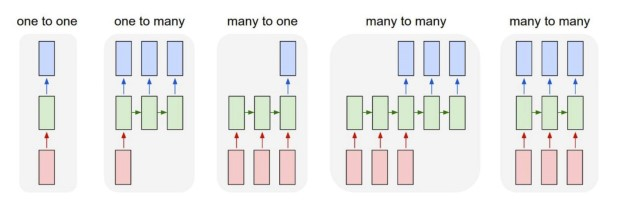
\includegraphics[scale = 1.5]{img/rnn2.jpg}
		\label{mi}
        \caption{Recurrent neural network}
\end{figure}

\begin{itemize}
    \item The \textbf{one-to-many} RNN is used for solving the \textbf{image captioning} problem;
    \item The \textbf{many-to-one} RNN is used for solving the \textbf{sentiment classification} problem (i.e., given a sequence of words, provide the sentiment);
    \item The \textbf{many-to-many} RNN is used for solving the \textbf{machine translation} problem (i.e., given a sequence of words, translating it into another sequence of words). The many-to-many is also used for \textbf{video classification}.
\end{itemize}

\subsubsection{Character-level Language Model}
An example of application of RNN is the character-level language model, in which the goal is to predict the following letter.

\begin{figure}[h!]
		\centering
        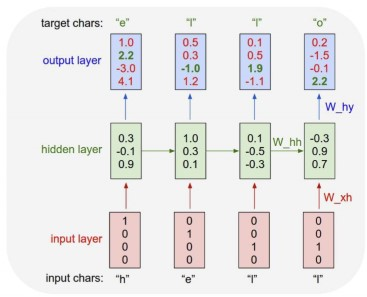
\includegraphics[scale = 1.5]{img/example rnn1.jpg}
		\label{mi}
        \caption{Character-level LM: training}
\end{figure}

As we can see, at test time the predictions at time $t$ are used for the predictions at time $t+1$.

\begin{figure}[h!]
		\centering
        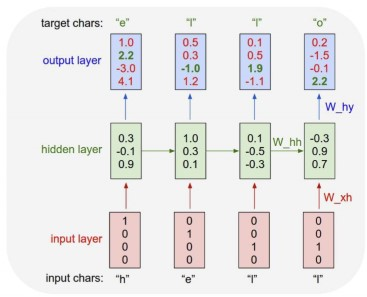
\includegraphics[scale = 1.5]{img/example rnn1.jpg}
		\label{mi}
        \caption{Character-level LM: test}
\end{figure}

However, one possible problems when dealing with RNN is the \textbf{vanishing gradient problem}, so a possible solution is to perform a \textbf{truncated back-propagation}: in this way, the error is backpropagated for a smaller number of steps.

\subsubsection{Image captioning}
We focus now on the image captioning problem: the idea here is to exploit a CNN (in this case AlexNet) to extract the features of an image, and then use these features for training a RNN which can solve the problem.

$$
\text{Image} \to \text{CNN} \to \text{RNN}
$$

\begin{figure}[h!]
		\centering
        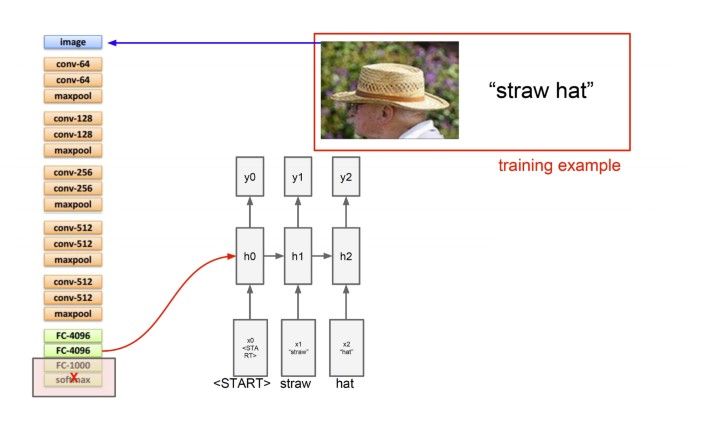
\includegraphics[scale = 1.5]{img/image captioning 1.jpg}
		\label{mi}
        \caption{Image captioning: training}
\end{figure}

As we can see, the last two layers are deleted, since we do not care about the actual classification of the image, but only on the feature the CNN extracted. Finally, the features are provided as input to the RNN, which returns the caption of the image. 

\begin{figure}[h!]
		\centering
        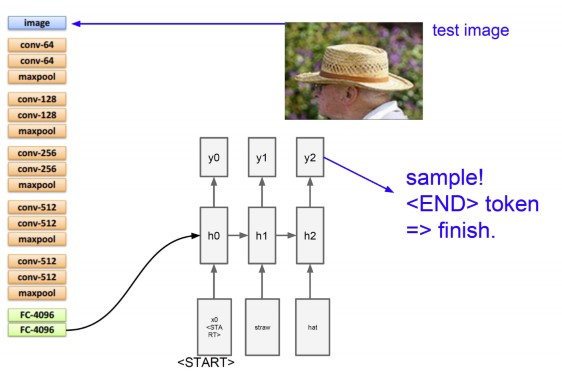
\includegraphics[scale = 1.5]{img/image captioning 2.jpg}
		\label{mi}
        \caption{Image captioning: test}
\end{figure}

At test time, an image without caption is provided as input to the CNN, the features are extracted, and then the RNN is used to provide the caption of the image.

\subsection{Some problems of CNN}
It was showed in several papers how adding some noise bring the Deep Neural Network to misclassify the input image, and this inspired a very important branch of ML, called \textbf{adversarial ML}.
